The tracking will typically have a few frames where either the particle is obstructed or is not detected correctly 
leading to spikes in the data. To make further theoretical analysis possible such points are removed manually. The basis for removal is simply a large discontinuity in the data, and could largely be eliminated with algorithmic means. However in particular for $n_z$ it's very difficult to write an algorithm that will satisfactory catch all possible edge cases. For example $n_z$ have peaks that make its derivative non continuous which means that cannot be use as a criterion. It's thus simpler to look at the analysis program and remove the points where the particle cannot be traced accurately due to noise. We will refer to this process as \emph{brushing}.

An example of unbrushed and brushed data can be seen in figure \ref{fig:brushed} and all unbrushed data files will be 
available at \url{http://goo.gl/jgzSXe}.

\begin{figure}[H]
\centering
\begin{subfigure}[3a]{0.40\textwidth}
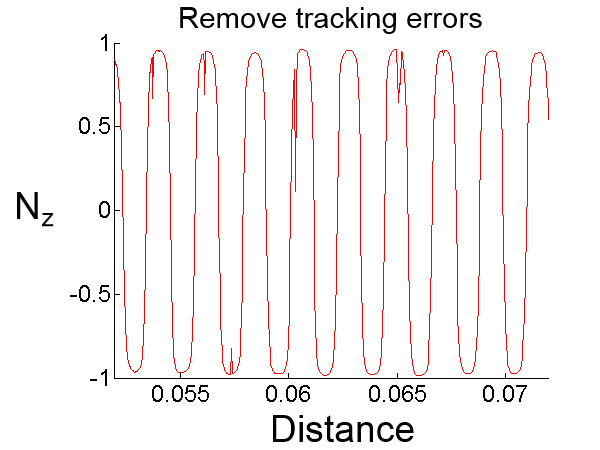
\includegraphics[width=\textwidth]{figures/method/Brushing1.png}
\caption{$n_x$ time series before brushing.}\label{fig:prebrush}
\end{subfigure}\hspace{1em}%
\begin{subfigure}[3b]{0.40\textwidth}
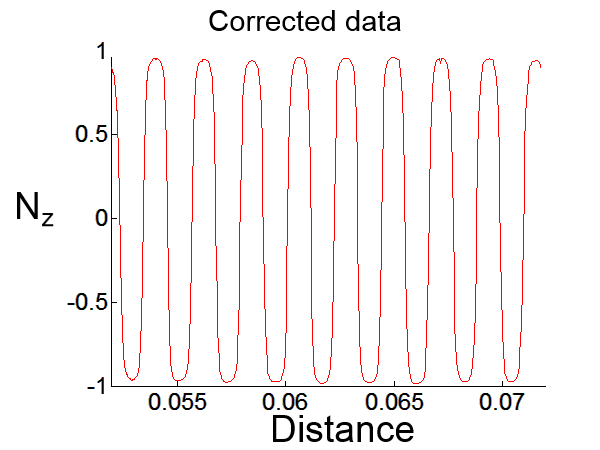
\includegraphics[width=\textwidth]{figures/method/Brushing2.png}
\caption{$n_x$ time series after brushing.}\label{fig:postbrush}
\end{subfigure} \\
\caption{Shows a time series of $n_x$ before and after removing points where a significant amount of noise disturbed the tracking. } \label{fig:brushed}
\end{figure}
